\section{Computational Companion}
\label{sec:ch1-computational-companion}

Analytical calculation remains the foundation of this chapter, but a short computational experiment can make geometry visible and can test algebra before it is used in a larger model. The examples below use NumPy for array operations and Matplotlib for visualization. Complete, runnable files are stored in \texttt{code/chapter01/python/}; Wolfram Language equivalents are collected in \texttt{code/chapter01/mathematica/chapter01\_companion.wl}.

\begin{physicalbox}[Computation as a check --- not a substitute]
A numerical result can verify a calculation for chosen inputs, reveal a sign error, or display a transformation. It does not replace a proof. For example, observing that two computed vectors are orthogonal to machine precision supports one calculation; the Gram--Schmidt derivation explains why orthogonality holds in general.
\end{physicalbox}

\subsection{Projection and Orthogonal Decomposition}
For vectors \(\mathbf a\) and nonzero \(\mathbf b\), the projection is
\[
\operatorname{proj}_{\mathbf b}\mathbf a
=\frac{\mathbf a\cdot\mathbf b}{\mathbf b\cdot\mathbf b}\mathbf b.
\]
The following program evaluates the formula and draws the parallel and perpendicular components.

\lstinputlisting[style=prbookpython,caption={Computing and visualizing an orthogonal projection.},label={lst:python-projection}]{code/chapter01/python/vector_projection.py}

\begin{figure}[H]
\centering
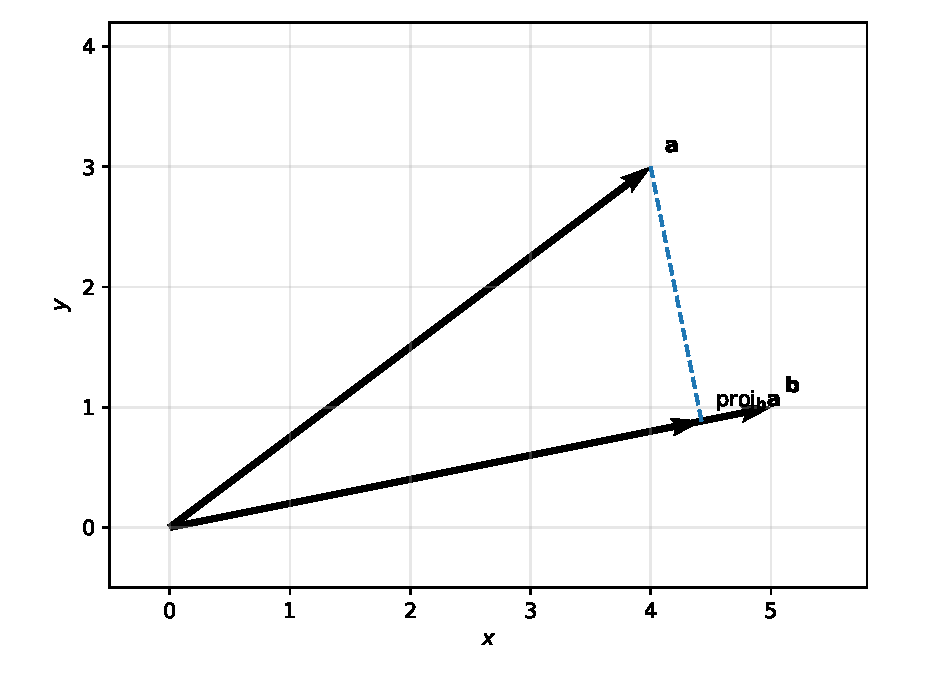
\includegraphics[width=0.72\textwidth]{figures/ch01/computational/vector_projection.pdf}
\caption{Numerical visualization of \(\mathbf a=\operatorname{proj}_{\mathbf b}\mathbf a+\mathbf a_\perp\). The dashed segment is perpendicular to \(\mathbf b\).}
\label{fig:computational-projection}
\end{figure}

\subsection{Rotations Preserve Lengths and Angles}
A counterclockwise rotation through \(\theta\) is represented by
\[
R(\theta)=
\begin{pmatrix}
\cos\theta&-\sin\theta\\
\sin\theta&\cos\theta
\end{pmatrix}.
\]
Because \(R^{\mathsf T}R=I\), one has \(\lVert R\mathbf v\rVert=\lVert\mathbf v\rVert\). The script below evaluates several rotations of the same vector.

\lstinputlisting[style=prbookpython,caption={Applying a rotation matrix to a vector.},label={lst:python-rotation}]{code/chapter01/python/rotation.py}

\begin{figure}[H]
\centering
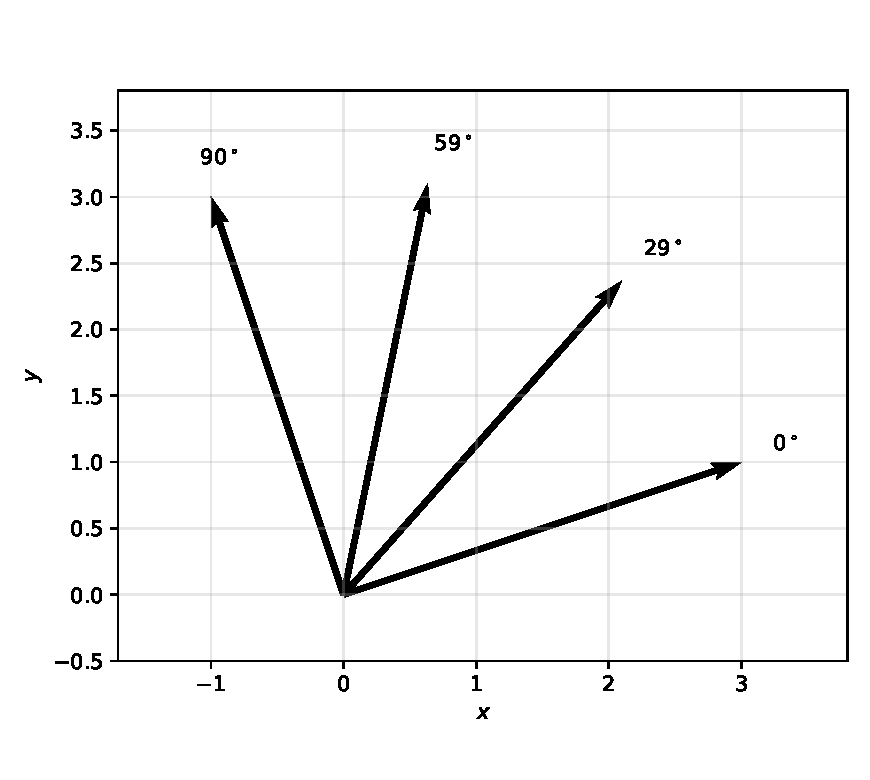
\includegraphics[width=0.68\textwidth]{figures/ch01/computational/rotation.pdf}
\caption{A vector rotated through several angles. Every arrow has the same length because an orthogonal rotation preserves the inner product.}
\label{fig:computational-rotation}
\end{figure}

\subsection{Linear Transformations of Shapes and Bases}
A matrix acts on every point of a geometric object and on the basis vectors used to describe it. Plotting both the original square and its image makes shear, stretch, and rotation immediately distinguishable.

\lstinputlisting[style=prbookpython,caption={Visualizing the action of a linear transformation.},label={lst:python-linear-map}]{code/chapter01/python/linear_transformation.py}

\begin{figure}[H]
\centering
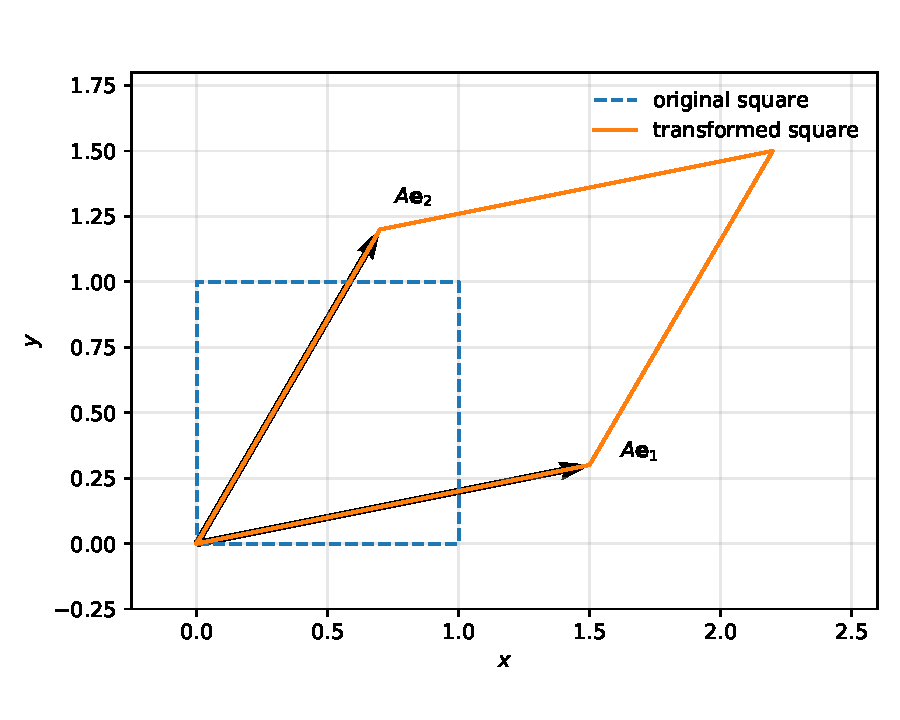
\includegraphics[width=0.72\textwidth]{figures/ch01/computational/linear_transformation.pdf}
\caption{A unit square and its image under a linear transformation. The transformed basis vectors are the columns of the matrix.}
\label{fig:computational-linear-map}
\end{figure}

\subsection{Gram--Schmidt Orthogonalization}
The Gram--Schmidt algorithm converts linearly independent vectors into an orthonormal basis. Numerically, the final dot product should be close to zero; small residual values arise from finite-precision arithmetic.

\lstinputlisting[style=prbookpython,caption={A two-dimensional Gram--Schmidt calculation.},label={lst:python-gram-schmidt}]{code/chapter01/python/gram_schmidt.py}

\begin{figure}[H]
\centering
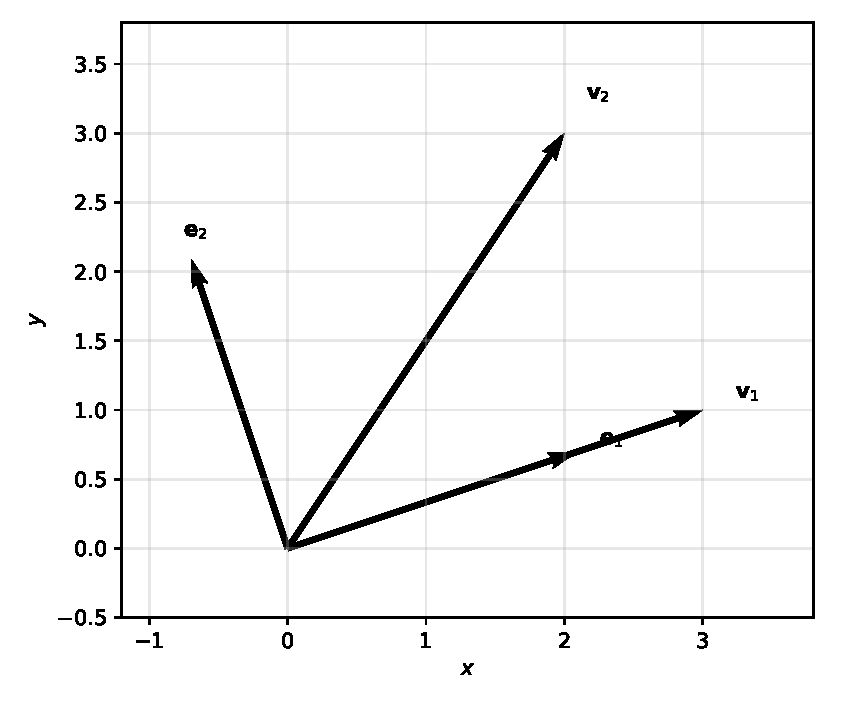
\includegraphics[width=0.68\textwidth]{figures/ch01/computational/gram_schmidt.pdf}
\caption{The original pair \(\mathbf v_1,\mathbf v_2\) and the orthonormal pair \(\mathbf e_1,\mathbf e_2\) produced by Gram--Schmidt.}
\label{fig:computational-gram-schmidt}
\end{figure}

\subsection{Wolfram Language Equivalents}
The same ideas can be explored symbolically. In Wolfram Language, \texttt{Orthogonalize} implements Gram--Schmidt, while matrix multiplication and graphics use nearly the same mathematical structure as the formulas in the text.

\lstinputlisting[style=prbookwolfram,caption={Projection, rotation, transformation, and orthogonalization in Wolfram Language.},label={lst:wolfram-ch1}]{code/chapter01/mathematica/chapter01_companion.wl}

\begin{mistakebox}[Common computational mistake]
Array multiplication is not universal across programming languages. In NumPy, \texttt{a @ b} denotes a matrix or dot product, while \texttt{a * b} multiplies components element by element. Always check the operation implemented by the language rather than inferring it from the printed symbols.
\end{mistakebox}
